\documentclass[border=0pt]{standalone}
\usepackage{tikz}
\usepackage{amsmath, amsthm, amssymb}
\usepackage{mathtools}
%\input{commondefinitions}
\usetikzlibrary{plotmarks}
\newcommand\marksymbol[2]{\tikz[#2,scale=1.2]\pgfuseplotmark{#1};}

\newcommand{\ind}[2]{\stackrel{\mathclap{\normalfont\mbox{\scriptsize #1}}}{#2}}

\colorlet{coscolor}{blue}
\newcommand{\cuadritotikz}{
% \pgfmathsetmacro{\unitstep}{5.2}
% \node at (-0.5,0.5) {(a)} ;
    \foreach \x in {0,1,2,3} {
      \foreach \y in {0,1,2,3} {
        \begin{scope}[shift={(\x,-\y)}] 
          \draw[black!10] (0,0) rectangle (1,1); 
%           \node at (0.5,0.5) {$\tau_{\y,\x}$};
         \end{scope}
%         \node[block] at (2,-\y) (block\y) {$f_\y$};
%         \draw[->] (block\y.east) -- +(0.5,0);
    }
    }
 \draw (0,-3) rectangle (4,1);
}

\begin{document}
\pagestyle{empty}
%\begin{tikzpicture}[x=0.8cm, y=0.8cm] % {{{
%\pgfmathsetmacro{\unitstep}{5.2}
%\begin{scope}[shift={(-1*\unitstep,0)}] 
%\node at (-0.5,0.5) {(a)};
%\begin{scope}[shift={(0,0)}] \fill[black] (0,0) rectangle (1,1); \end{scope}
%\begin{scope}[shift={(0,0)}] 
%	\draw[black!10] (0,0) rectangle (1,1); 
%	\node at (0.5,0.5) {\scalebox{1}{\textcolor{white}{$\tau_{\ind{00}{00}}$}}};
%\end{scope}
%\begin{scope}[shift={(3,0)}] \fill[black] (0,0) rectangle (1,1); \end{scope}
%\begin{scope}[shift={(3,0)}] 
%	\draw[black!10] (0,0) rectangle (1,1); 
%	\node at (0.5,0.5) {\scalebox{1}{\textcolor{white}{$\tau_{\ind{00}{11}}$}}};
%\end{scope}
%\begin{scope}[shift={(3,-3)}] \fill[black] (0,0) rectangle (1,1); \end{scope}
%\begin{scope}[shift={(3,-3)}] 
%	\draw[black!10] (0,0) rectangle (1,1); 
%	\node at (0.5,0.5) {\scalebox{1}{\textcolor{white}{$\tau_{\ind{11}{11}}$}}};
%\end{scope}
%\begin{scope}[shift={(0,-3)}] \fill[black] (0,0) rectangle (1,1); \end{scope}
%\begin{scope}[shift={(0,-3)}] 
%	\draw[black!10] (0,0) rectangle (1,1); 
%	\node at (0.5,0.5) {\scalebox{1}{\textcolor{white}{$\tau_{\ind{11}{00}}$}}};
%\end{scope}
%\draw (0,-3) rectangle (4,1);
%\end{scope} % }}}
%\end{tikzpicture} % }}}
%
%
%
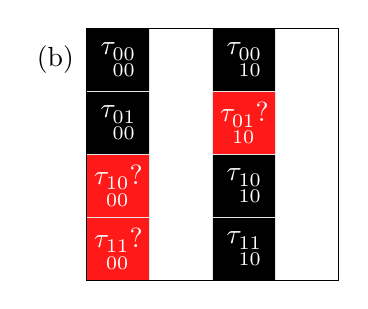
\begin{tikzpicture}[x=0.8cm, y=0.8cm] % {{{
\pgfmathsetmacro{\unitstep}{5.2}
\begin{scope}[shift={(-1*\unitstep,0)}] 
\node at (-0.5,0.5) {(b)};
\begin{scope}[shift={(0,0)}] \fill[black] (0,0) rectangle (1,1); \end{scope}
\begin{scope}[shift={(0,0)}] 
	\draw[black!10] (0,0) rectangle (1,1); 
	\node at (0.5,0.5) {\scalebox{1}{\textcolor{white}{$\tau_{\ind{00}{00}}$}}};
\end{scope}
\begin{scope}[shift={(2,0)}] \fill[black] (0,0) rectangle (1,1); \end{scope}
\begin{scope}[shift={(2,0)}] 
	\draw[black!10] (0,0) rectangle (1,1); 
	\node at (0.5,0.5) {\scalebox{1}{\textcolor{white}{$\tau_{\ind{00}{10}}$}}};
\end{scope}
\begin{scope}[shift={(0,-1)}] \fill[black] (0,0) rectangle (1,1); \end{scope}
\begin{scope}[shift={(0,-1)}] 
	\draw[black!10] (0,0) rectangle (1,1); 
	\node at (0.5,0.5) {\scalebox{1}{\textcolor{white}{$\tau_{\ind{01}{00}}$}}};
\end{scope}
\begin{scope}[shift={(2,-2)}] \fill[black] (0,0) rectangle (1,1); \end{scope}
\begin{scope}[shift={(2,-2)}] 
	\draw[black!10] (0,0) rectangle (1,1); 
	\node at (0.5,0.5) {\scalebox{1}{\textcolor{white}{$\tau_{\ind{10}{10}}$}}};
\end{scope}
\begin{scope}[shift={(2,-3)}] \fill[black] (0,0) rectangle (1,1); \end{scope}
\begin{scope}[shift={(2,-3)}] 
	\draw[black!10] (0,0) rectangle (1,1); 
	\node at (0.5,0.5) {\scalebox{1}{\textcolor{white}{$\tau_{\ind{11}{10}}$}}};
\end{scope}
\begin{scope}[shift={(2,-1)}] \fill[red!90] (0,0) rectangle (1,1); \end{scope}
\begin{scope}[shift={(2,-1)}] 
	\draw[black!10] (0,0) rectangle (1,1); 
	\node at (0.5,0.5) {\scalebox{1}{\textcolor{white}{$\tau_{\ind{01}{10}}$?}}};
\end{scope}
\begin{scope}[shift={(0,-2)}] \fill[red!90] (0,0) rectangle (1,1); \end{scope}
\begin{scope}[shift={(0,-2)}] 
	\draw[black!10] (0,0) rectangle (1,1); 
	\node at (0.5,0.5) {\scalebox{1}{\textcolor{white}{$\tau_{\ind{10}{00}}$?}}};
\end{scope}
\begin{scope}[shift={(0,-3)}] \fill[red!90] (0,0) rectangle (1,1); \end{scope}
\begin{scope}[shift={(0,-3)}] 
	\draw[black!10] (0,0) rectangle (1,1); 
	\node at (0.5,0.5) {\scalebox{1}{\textcolor{white}{$\tau_{\ind{11}{00}}$?}}};
\end{scope}
\draw (0,-3) rectangle (4,1);
\end{scope} % }}}
\end{tikzpicture} % }}}
\end{document}
